\chapter{Objetivos del proyecto}

\section{Definición del proyecto}

\subsection{Objetivos}

La gestión de repositorios semánticos compatibles con el estándar \acrshort{oaipmh} tiene como objetivo explotar la información almacenada en un repositorio de manera más eficiente, mediante consultas semánticas y facetadas avanzadas. Busca dar soporte a \acrshort{oaipmh} para disponer de todo el contenido según dicta su estándar.

Como caso práctico se propone añadir compatibilidad con \acrshort{oaipmh} al sistema de gestión de grupos de investigación LabMan, para que pueda proveer de datos a clientes que trabajen con esta tecnología.

Para dar sentido a esta funcionalidad, se pretende expandir labman con un cliente que se alimente con estos recursos para ofrecer servicios orientados a la búsqueda semántica y facetada.
\subsection{Alcance del proyecto}

Atendiendo a las premisas señaladas anteriormente, las funcionalidades que deberá soportar este proyecto serán:

\begin{itemize}
	\item Un servidor capaz de conectarse al repositorio de \acrshort{labman} y extraer la información actualizada, en forma de metadatos, sobre las publicaciones y sus autores correspondientes de acuerdo con el estándar \acrlong{dc}\cite{DC}, respondiendo a las peticiones \acrshort{http} de acuerdo con el protocolo \acrshort{oaipmh}.
	
	\item Un cliente web que extienda \acrshort{labman} capaz de realizar busquedas y filtros complejos sobre los proyectos y publicaciones mediante un proceso intuitivo para los usuarios, compuesto por formularios que se dispondrán de forma sencilla en primera instancia, para dar la posibilidad de realizar consultas rápidas y simples sin abrumar a los usuarios por la longitud del mismo. Pero, a su vez, han de permitir dar la posibilidad de expandir los campos con el fin de introducir datos más específicos para realizar consultas más elaboradas.

	\item La plataforma estará diseñada de una manera intuitiva, para que así, personas con pocos conocimientos de la informática también la puedan usar sin ningún tipo de problema. Además ha de ser responsiva, es decir, su diseño se adaptará a distintos tamaños de pantallas como pueden ser las de un ordenador de sobremesa, un portátil, una tableta o un móvil, donde poder plasmar toda la información de una manera legible para los humanos.
\end{itemize}
\subsection{Producto final}

El producto final se compone de dos sistemas diferentes:

El primero es un servidor de documentos \acrfull{xml}\cite{XML} en el esquema \acrshort{dc}, capaz de responder a las peticiones \acrshort{html} según el protocolo \acrshort{oaipmh}. Será capaz de proveer información variada acerca de las publicaciones de los miembros que conforman MORElab en DeustoTech.

Los datos que proporcionará serán una relación de las tablas del repositorio de \acrshort{labman} acerca de las publicaciones pudiendo ser:

\begin{itemize}
	\item Actas.
	\item Ponencias.
	\item Tesis doctorales.
	\item Artículos de revistas.
	\item Artículos de publicaciones.
	\item Libros.

\end{itemize}

La segunda es una aplicación web que permita a todo el mundo consultar y filtrar la información, de forma esquematizada y ordenada, sobre las publicaciones y proyectos del equipo de investigación de MORElab por medio de sus atributos más significativos a través de formularios dinámicos e interactivos.

\section{Descripción de realización}

\subsection{Método de desarrollo}

El proyecto se desarrollará mediante un sistema de fases, en las que el orden es algo vital puesto que cada una de las fases dependerá de la previa, en el \acrfull{edt} (figura \ref{fig:edt}) puede verse su estructura.

\begin{figure}[!htp]
	\centering
	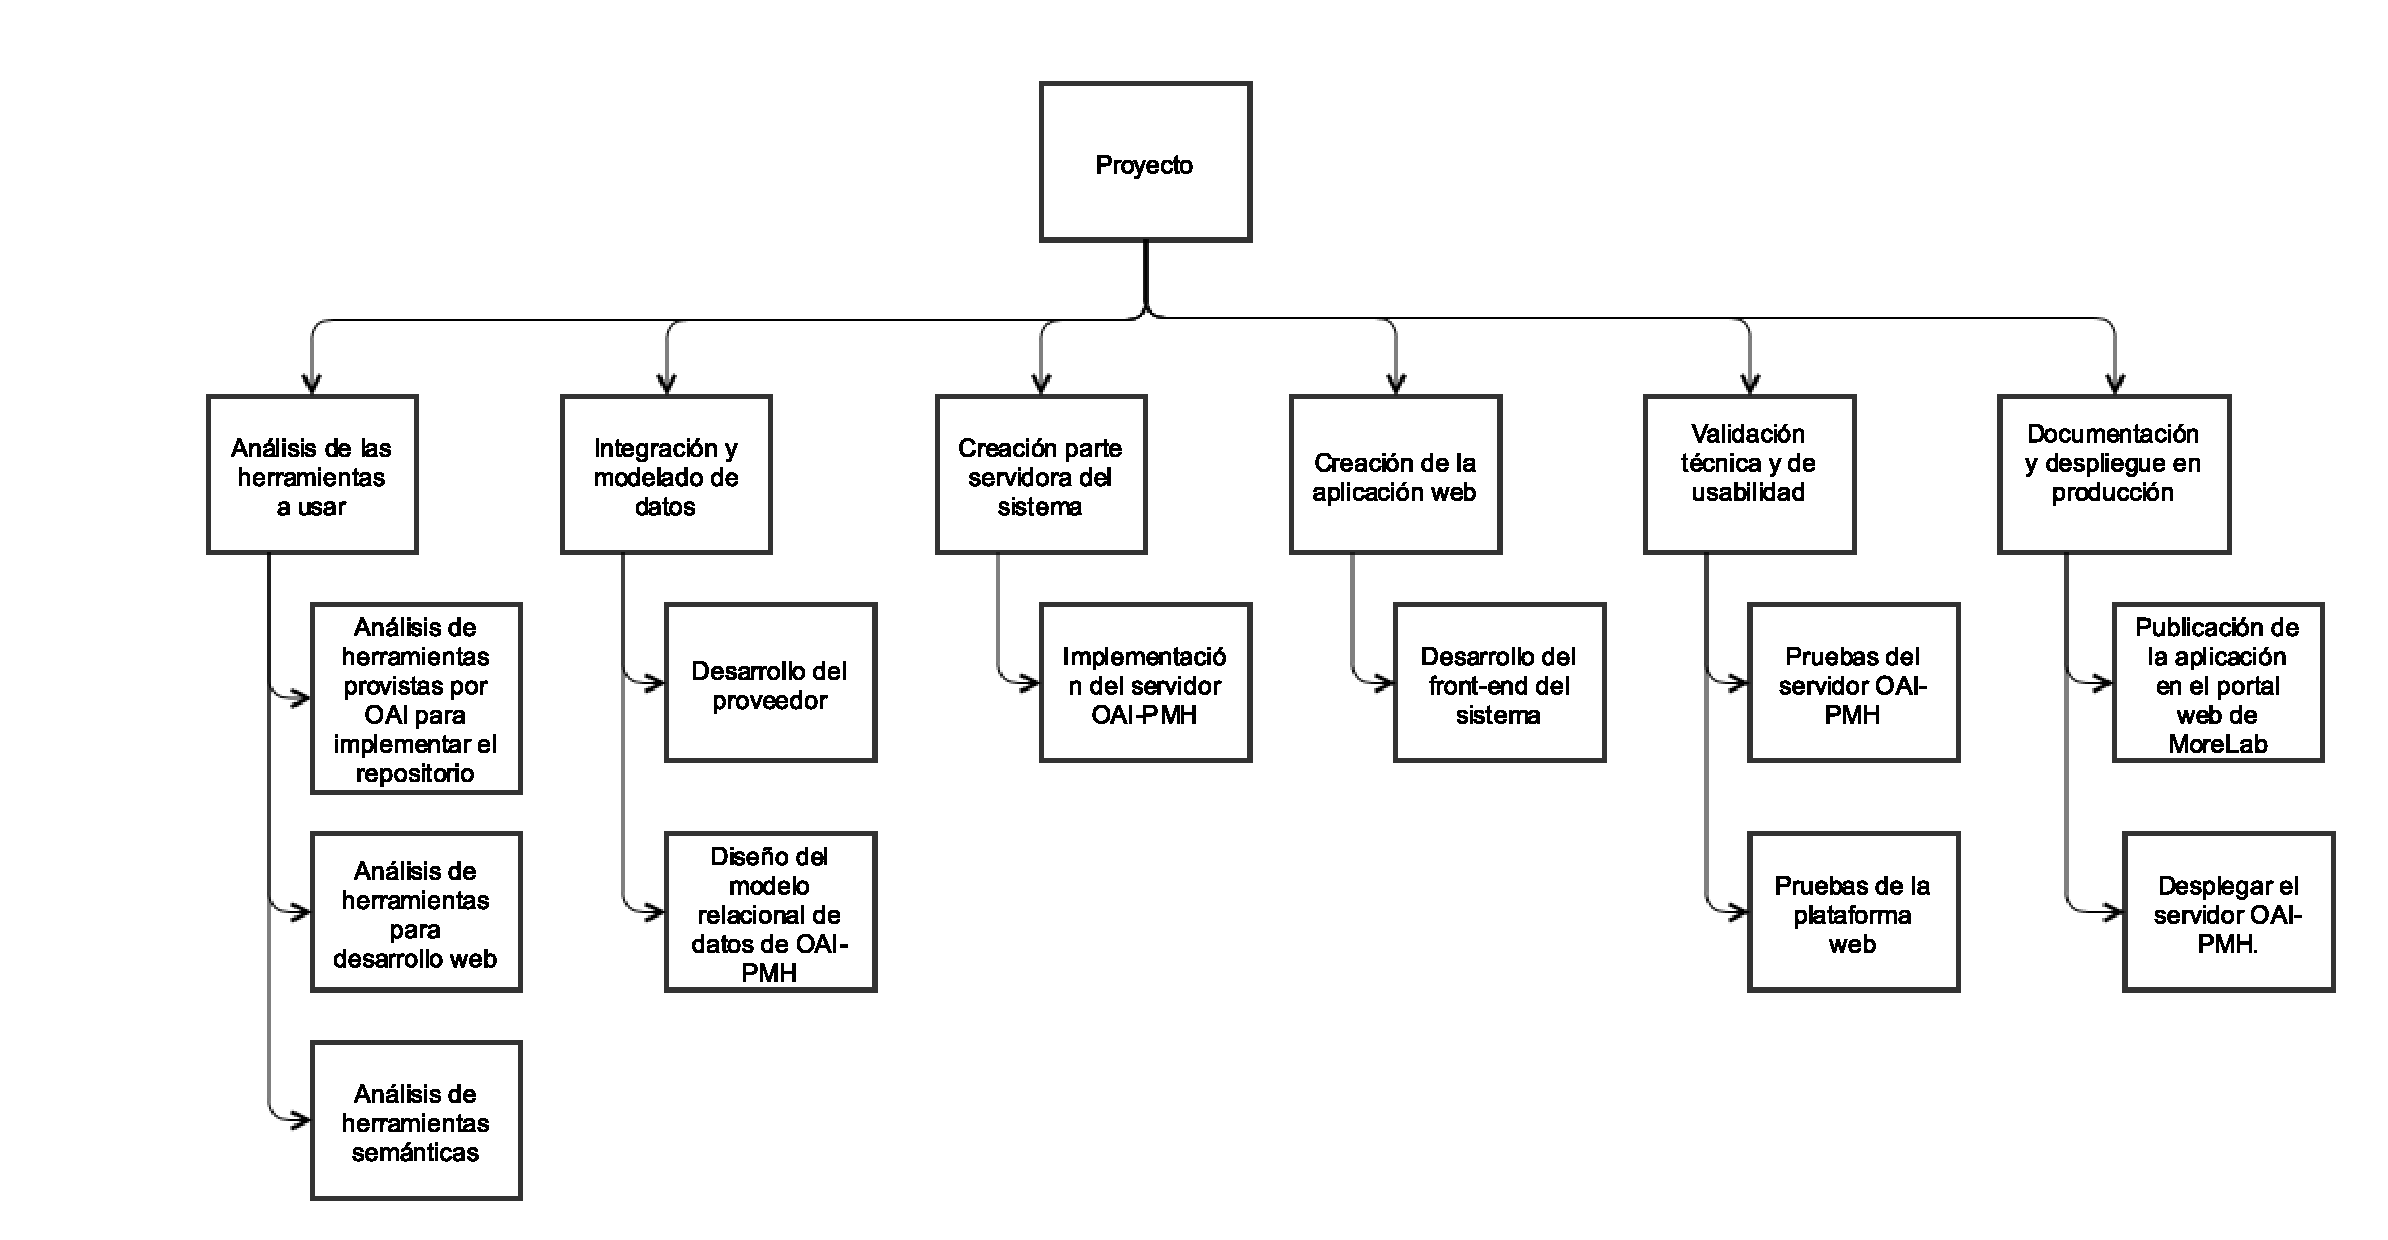
\includegraphics[angle=-90, scale=.5]{fig/edt}
	\caption{EDT}\label{fig:edt}
\end{figure}

Por tanto, las fases de la solución planteada serán las siguientes:

\begin{enumerate}
	\item \textbf{Análisis de las herramientas a usar:}

	En esta fase se analizarán todas las posibles herramientas que se pueden usar para el desarrollo del proyecto y se elegirán las más adecuadas de acuerdo a las necesidades del proyecto y a los conocimientos del equipo de trabajo.
	\item \textbf{Integración y modelado de datos:}

	Es la fase en la que se identificará y seleccionarán las tablas del repositorio de las que se extraerá la información para su adaptación a Dublin Core.
	\item \textbf{Creación del servidor de OAI-PMH:}

	Diseño e implementación servidor.
	\item \textbf{Creación de la aplicación web:}

	Diseño e implementación del front-end de la aplicación web. 
	\item \textbf{Validación técnica y de usabilidad:}

	Es la fase donde se realizarán las pruebas finales del sistema completo.
	\item \textbf{Documentación y despliegue en producción:}

	Es donde se terminará de redactar la documentación necesaria y se desplegará el producto.
\end{enumerate}
\subsection{Productos intermedios}

Los productos intermedios que se generarán en cada una de las fases son:

\begin{itemize}
	\item \textbf{Integración y modelado de datos:}
	\begin{itemize}
		\item Especificación y diseño de la base de conocimiento del servidor \acrshort{oaipmh}.
	\end{itemize}
	\item \textbf{Creación parte servidora del sistema:}
	\begin{itemize}
		\item Módulo de proveedor de la base de conocimiento.
		\item Módulo de adaptación y almacenamiento del conocimiento en \acrlong{dc}.
		\item Módulo de servicio de \acrshort{xml}.
	\end{itemize}
	\item \textbf{Creación de la aplicación web:}
	\begin{itemize}
		\item Aplicación web del sistema.
	\end{itemize}
	\item \textbf{Validación técnica y de usabilidad:}
	\begin{itemize}
		\item Informe de evaluación del sistema.
	\end{itemize}
\end{itemize}

\subsection{EDT}

\begin{figure}[!htp]
	\centering
	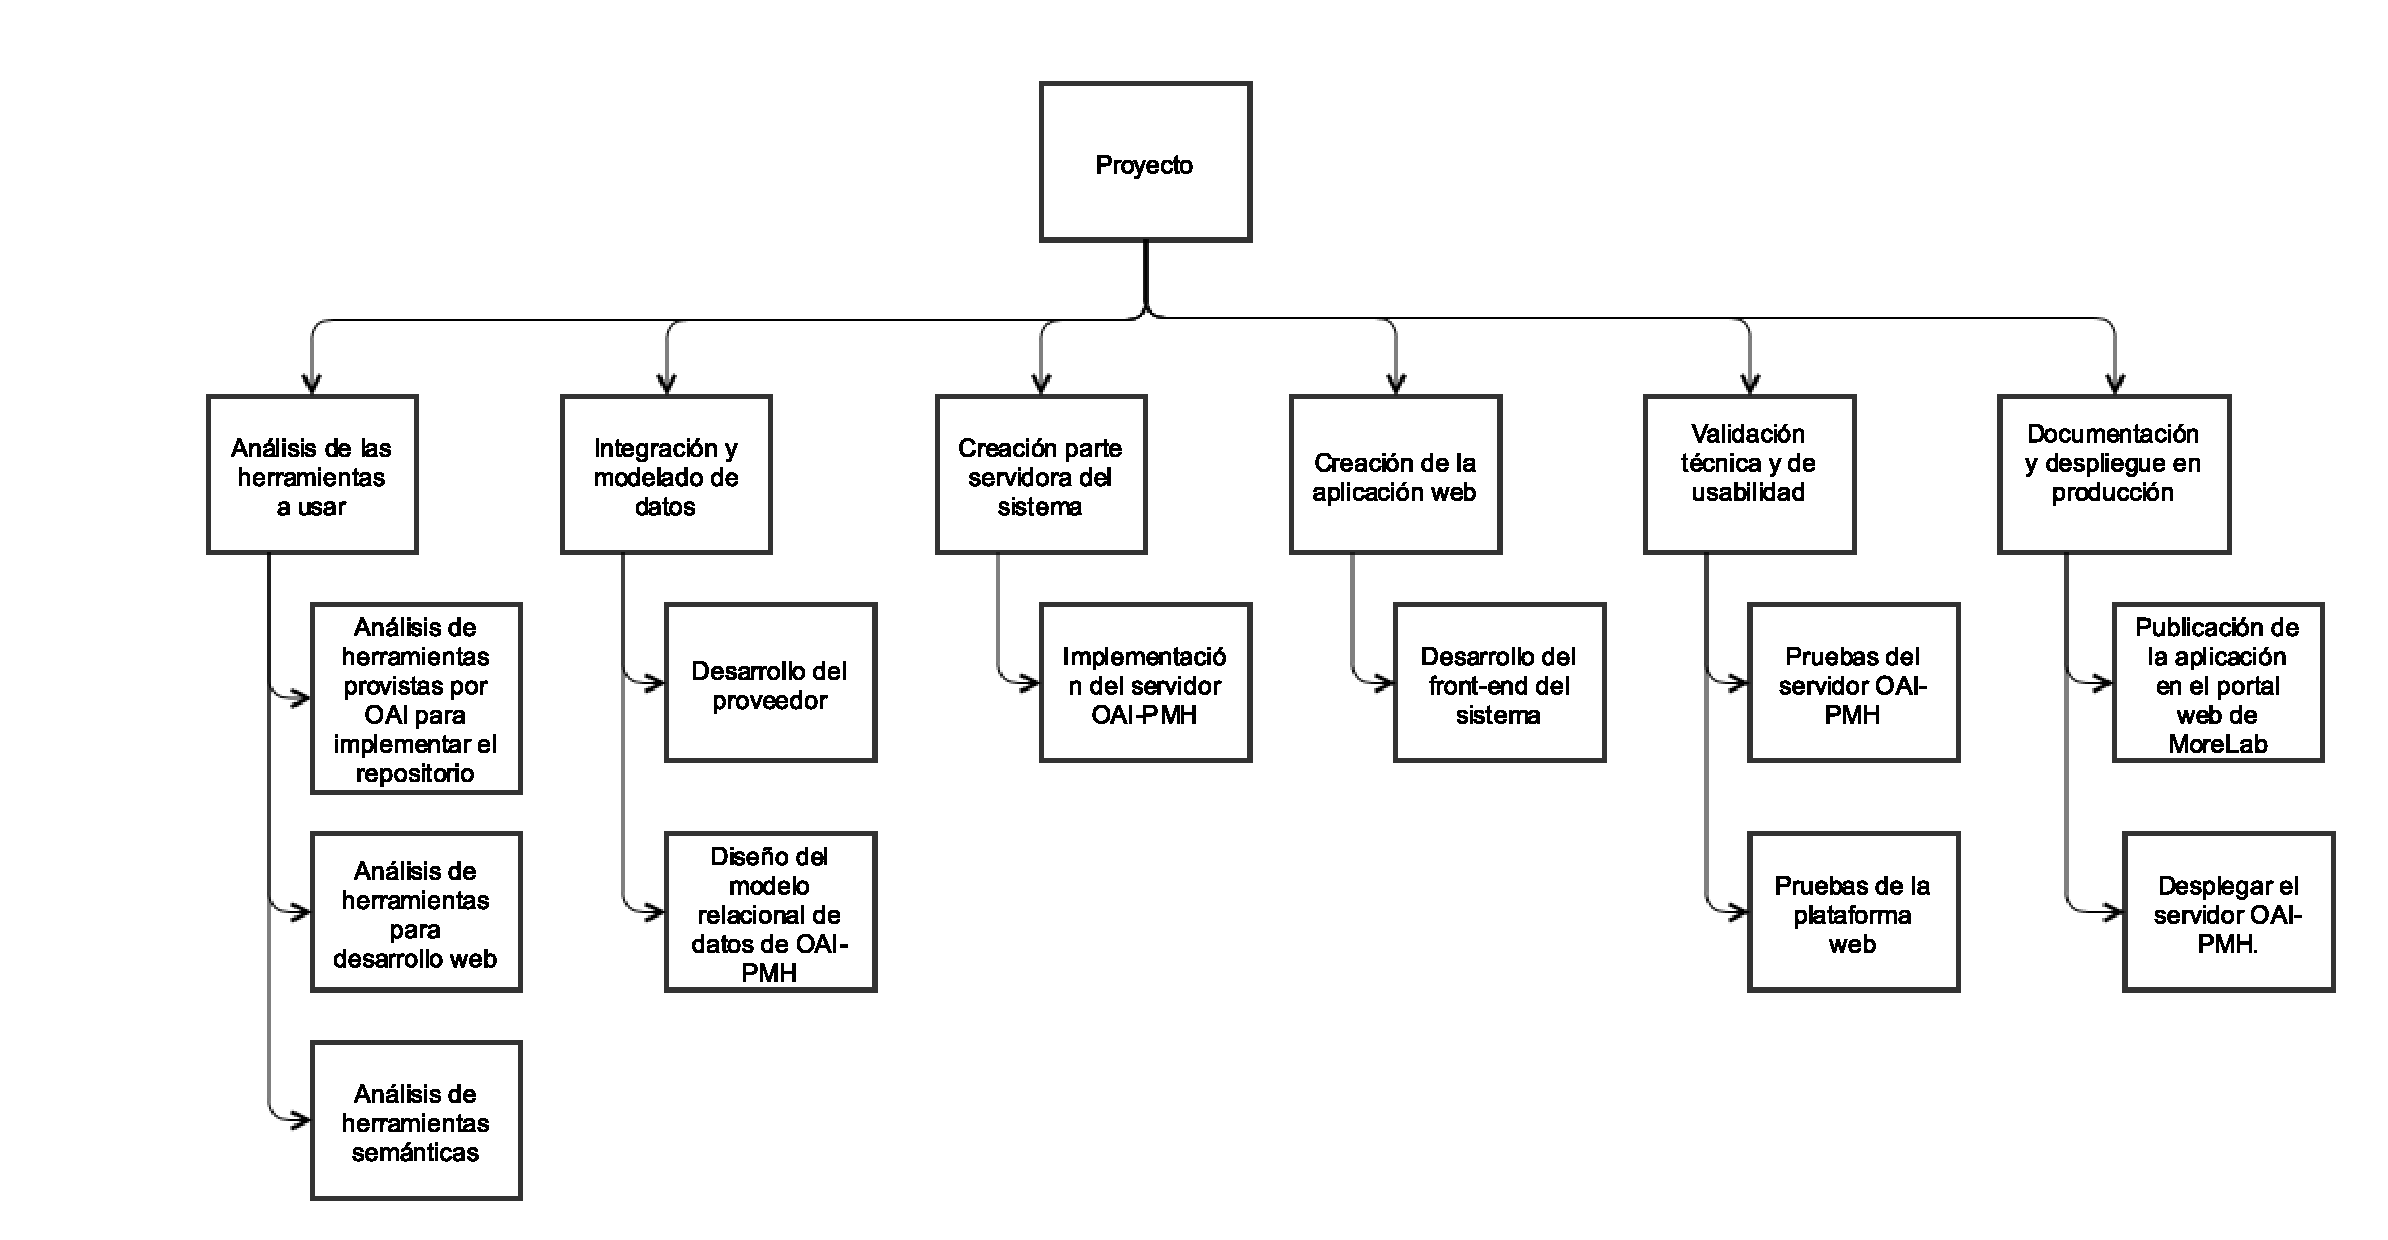
\includegraphics[angle=-90, scale=.5]{fig/edt}
	\caption{EDT}
\end{figure}

\subsection{Tareas principales}

La implantación del proyecto comprende las siguientes tareas o actividades: 

\subsubsection{Análisis de las herramientas a usar:}

\begin{itemize}
	\item \textbf{Análisis de herramientas provistas por \acrshort{oai} para implementar los requisitos mínimos para repositorio del protocolo \acrshort{oaipmh}.}

	Investigar las distintas alternativas que hay para crear un servidor que beba de distintos tipos repositorios.
	\item \textbf{Análisis de herramientas para desarrollo web.}

	Investigar las distintas herramientas que hay para el desarrollo web y que sean adecuadas para el propósito del proyecto.
	\item \textbf{Análisis de herramientas semánticas.}

	Investigar las distintas alternativas para realizar búsquedas según los estándares de la web semántica. 
\end{itemize}

\subsubsection{Integración y modelado de datos:}

\begin{itemize}
	\item \textbf{Desarrollo del proveedor.}
	
	Desarrollo del sistema de extracción de datos de las tablas necesarias del repositorio PostgreSQL.

	\begin{enumerate}
		\item Formación: aprendizaje en el uso de las herramientas.
		\item Diseño: diseño del sistema de extracción de datos.
		\item Implementación: programación del sistema de extracción de datos.
		\item Pruebas: pruebas del sistema de extracción de datos.
	\end{enumerate}
	\item \textbf{Diseño del modelo relacional de datos de \acrshort{oaipmh}.}
	\begin{enumerate}
		\item Diseño: diseño del modelo de la base de datos. 
		\item Implementación: inserción del modelo de datos en la base de datos.
		\item Pruebas: pruebas de la base de datos junto con el sistema de extracción de datos.
	\end{enumerate}
\end{itemize}

\subsubsection{Creación parte servidora del sistema:}

\begin{itemize}
	\item Implementación del servidor \acrshort{oaipmh}.

	Puesta en marcha del servidor \acrshort{oaipmh} que transforma datos almacenados mediante un modelo relacional a \acrshort{dc}.

	\begin{enumerate}
		\item Implementación: configuración del servidor.
		\item Pruebas: pruebas del servidor.
	\end{enumerate}
\end{itemize}

\subsubsection{Creación de la aplicación web:}

\begin{itemize}
	\item \textbf{Desarrollo del front-end del sistema.}
	\begin{enumerate}
		\item Formación en la herramienta de desarrollo web.
		\item Diseño básico de la plataforma web.
		\item Diseño del módulo de búsqueda avanzada de proyectos.
		\item Diseño del módulo de búsqueda avanzada de publicaciones.
	\end{enumerate}	
\end{itemize}

\subsubsection{Validación técnica y de usabilidad:}

\begin{itemize}
	\item \textbf{Pruebas del servidor \acrshort{oaipmh}.}
	\item \textbf{Pruebas de la plataforma web.}
\end{itemize}

\subsubsection{Documentación y despliegue en producción:}

\begin{itemize}
	\item \textbf{Publicación de la aplicación en el portal web de MoreLab.}
	
	Instalar la aplicación web en el servidor de LabMan y publicarlo en el portal web.
	\item \textbf{Desplegar el servidor \acrshort{oaipmh}.}

	Instalar el servidor \acrshort{oaipmh}, recolectar y exportar la información del repositorio.
\end{itemize}

\section{Organización y equipo}

\subsection{Esquema organizativo}

La organización del proyecto se articula en torno al comité de dirección y al equipo de trabajo que se va a encargar de desarrollar el producto, en función de la estructura de la figura \ref{fig:org_schema}.

\begin{itemize}
	\item \textbf{Comité de dirección:} su función principal es orientar por dónde debería ir el proyecto y tomar las decisiones finales a la hora de qué hacer o no. Además, este comité deberá aprobar las diferentes fases del proyecto.
	\item \textbf{Equipo de trabajo:} el órgano encargado de diseñar y desarrollar el contenido del proyecto en función de las diferentes fases estipuladas.
	\item \textbf{Seguimiento:} Debido a el bajo número de personas que compone el equipo de desarrollo se ha acordado trabajar mediante reuniones de seguimiento semanales pero también tras terminar cada tarea. En las reuniones semanales se reunirán todos los miembros del equipo, mientras que en las que corresponden a una tarea finalizada lo harán solo los que han participado en dicha tarea junto a el director de proyecto. Su finalidad será comentar los avances y/o problemas que hayan podido ocurrir, aunque también servirán para que el director de el visto bueno a la tarea y pasar a la siguiente. 
\end{itemize}

\begin{figure}[!htp]
	\centering
	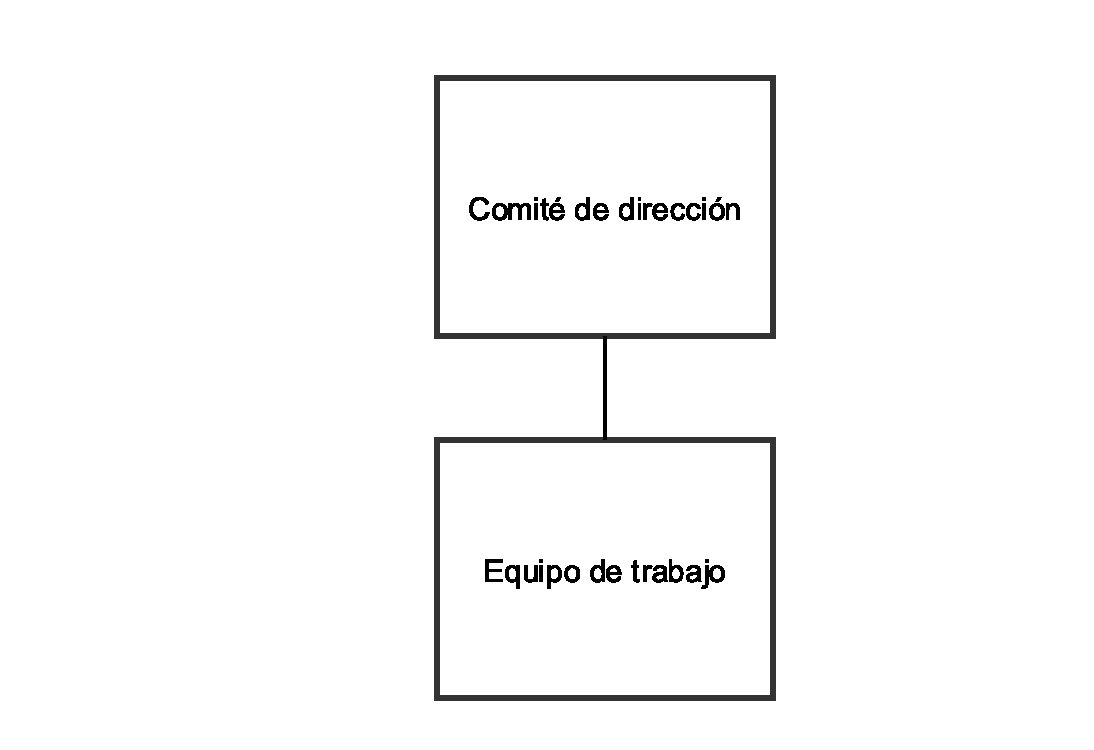
\includegraphics[scale=.75]{fig/organization}
	\caption{Esquema organizativo}\label{fig:org_schema}
\end{figure}
\subsection{Plan de Recursos Humanos}\label{sec:planRecursosHumanos}

El equipo de trabajo estará formado por los siguientes perfiles directamente relacionados con las diferentes áreas de competencias que se abordan en el proyecto: 

\begin{itemize}
	\item \textbf{Jefe de proyecto:} su función es realizar las actividades de organización, coordinación y seguimiento del proyecto.
	\item \textbf{Administrador de \acrlong{bd}}: su función es la de gestionar de una manera óptima la base de datos PostgreSQL y SPARQL además de colaborar en el estudio sobre las ventajas e inconvenientes tres tecnologías \acrshort{sql}, \acrshort{sparql} y acrshort{oaipmh}. 
	\item \textbf{Programador:} su función es la desarrollar toda la lógica del programa como la implementación de la plataforma web. 
	\item \textbf{Diseñador:} su función es la diseñar interfaces intuitivas para el usuario y adaptables para distintos dispositivos (portátiles, tablets, móviles) 
	\item \textbf{Experto en web semántica:} su función es ayudar en las cuestiones sobre la implementación de \acrshort{labman} relacionadas con la web semántica y colaborar en el estudio sobre las ventajas e inconvenientes tres tecnologías \acrshort{sql}, \acrshort{sparql} y acrshort{oaipmh}.
\end{itemize}

\section{Condiciones de ejecución}

\subsection{Entorno de trabajo}

El lugar de trabajo habitual serán las instalaciones de DeustoTech, aunque también se trabajará en casa para poder terminar a tiempo el proyecto.

El calendario y horario serán los correspondientes a los lugares de trabajo anteriormente mencionados durante una jornada laboral de aproximadamente 4 horas al día. Este horario podría verse modificado si se requiriera con el fin de cumplir los plazos establecidos.

En principio el director de proyecto será el responsable de todos los productos del desarrollo, y deberá dar el visto bueno a las herramientas que serán utilizadas para preservar las copias de seguridad y de definir cada cuanto tiempo deberán hacerse. En caso de que los desarrolladores no cumplan con estos requisitos y de producirse una perdida en el desarrollo serán estos los que asuman la responsabilidad, teniendo que optar por realizar horas extra o asumir de su sueldo la penalización que llegase a imponer el cliente en caso de no poder cumplirse con los plazos.

Los medios informáticos para la ejecución del proyecto deberán ser provistos por DeustoTech o serán los ordenadores personales de los integrantes del equipo. DeustoTech será responsable de todos los productos provistos para el desarrollo, salvo de aquellos medios pertenecientes a los propios desarrolladores. Los medios son los siguientes: 

\begin{itemize}
	\item Hardware
	\begin{itemize}
		\item Macbook Pro Retina 2012
		\item Servidor del repositorio Linux
		\item Monitor secundario
	\end{itemize}
	\item Software
	\begin{itemize}
		\item Licencia Sublime Text 2
		\item OS X
		\item Office 2011
		\item PostgreSQL
		\item SPARQL
	\end{itemize}
\end{itemize}
\subsection{Control de cambios}

Todas las peticiones que impliquen cambios en el diseño o en lo que ya está desarrollado, serán estudiadas y solo seguirán adelante si son modificaciones razonables y que son posibles de hacer dentro del plazo acordado. El procedimiento que habrá que seguir a la hora de  solicitar un cambio será:

\begin{enumerate}
	\item Comunicación de DeustoTech de las modificaciones solicitadas.
	\item Valoración por el equipo del proyecto de la repercusión técnica y cambios de plazos.
	\item Presentación de la decisión tomada por el equipo a DeustoTech.
	\item Notificación por parte de DeustoTech de la aprobación o no de la propuesta.	
	\item En caso afirmativo, modificación del plan de trabajo y del presupuesto.
\end{enumerate}
\subsection{Recepción de productos}

Para la recepción de productos, el equipo del proyecto definirá una serie de pruebas que serán estrictamente ejecutadas. Una vez pasadas las pruebas, el jefe de proyecto deberá revisar y aceptar el producto para poder presentarlo oficialmente a DeustoTech.  En caso de que exista algún problema tras la revisión,  la dirección de DeustoTech-Internet deberá comunicarlo en un plazo máximo de 5 días para poder llevar a cabo las modificaciones y así poder seguir con la siguiente fase del proyecto. En caso de no obtener respuesta en el intervalo de tiempo especificado anteriormente, se considerará aprobado.